Consider the second order problem

$$u''(x)=xu(x),\;\;\;x\geq0$$

which has a unique solution $u(x)$ with $u(\infty)=0$. Numerically find the solution approaching as
either a BVP or an IVP.

\begin{solution}\renewcommand{\qedsymbol}{}\ \\
    To solve the Airy equation, we took the approach of an IVP. Here, we set the initial values to be
    close to zero, on the order of about half of the epsilon in Matlab. That is, we set the initial
    conditions to be on the order of $10^{-6}$. From there, we simply used two already defined Matlab
    functions to approximate the solution to the equation. We used an in name only modified ode function
    as well as ode45. The approximate solution has the condition $u(\infty)=0$ as desired which can be
    seen below. SInce the solution is unique and the desired condition is met, we have a decent
    approximation.\\
    \begin{center}
        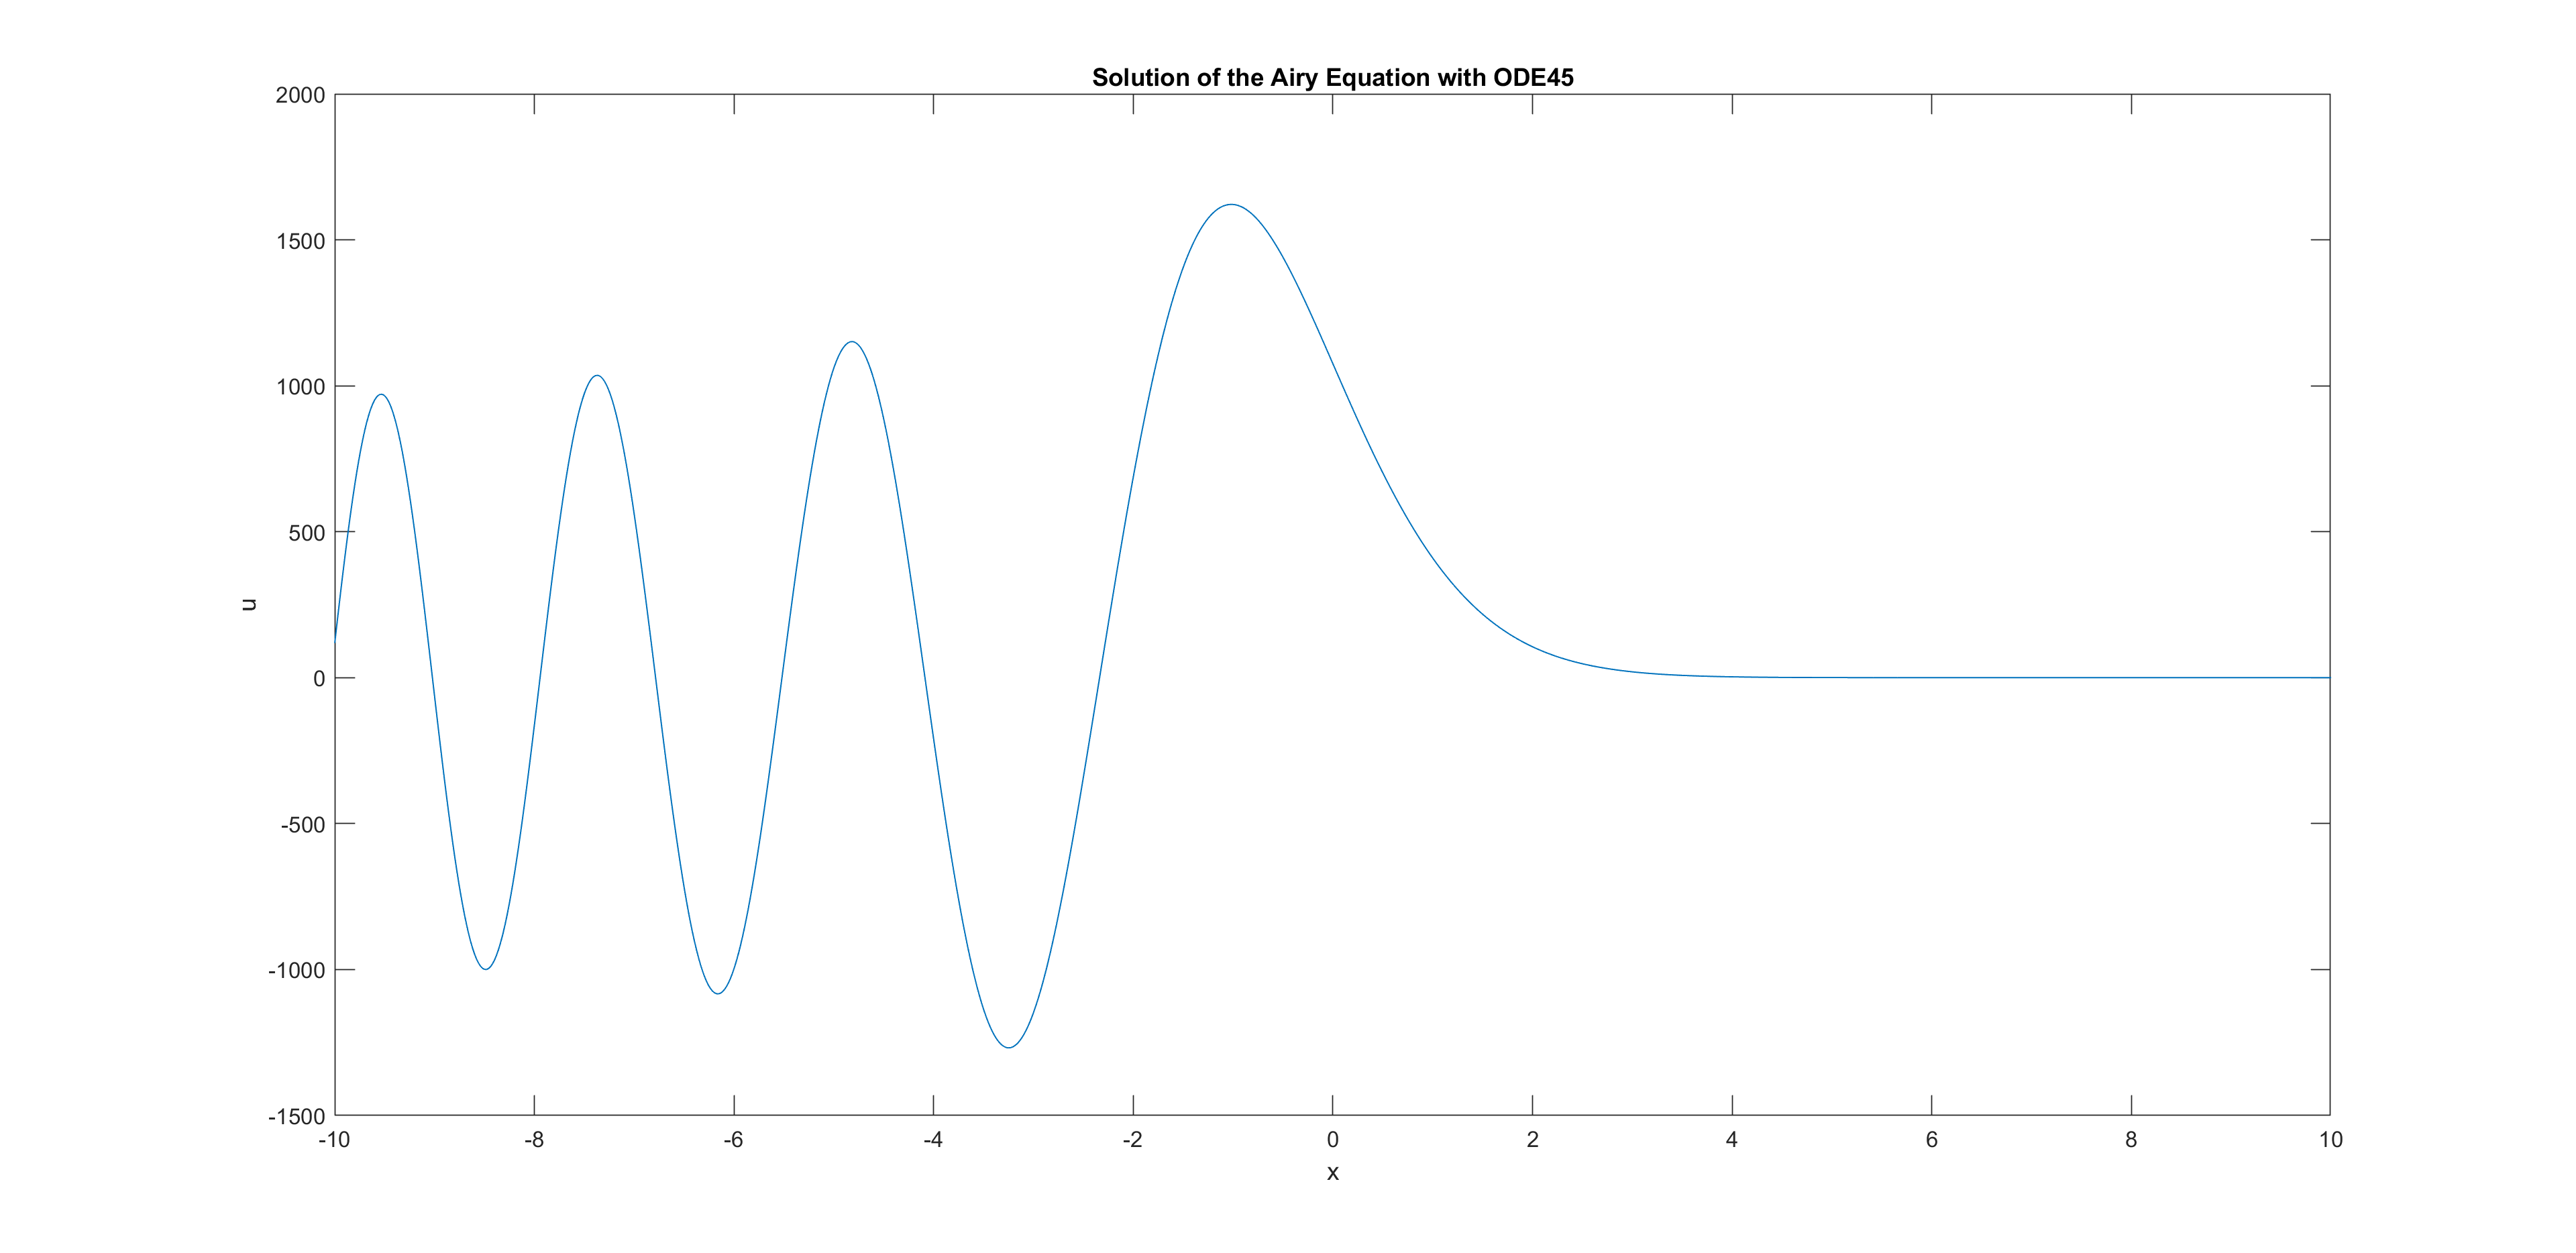
\includegraphics[scale=0.15]{4.PNG}
    \end{center}

\end{solution}

\newpage
\lstinputlisting{num4.m}